\documentclass[../ai_in_finance]{subfiles}
\usepackage[margin=1in]{geometry}
\usepackage{tikz}
\usetikzlibrary{positioning}
\usepackage{amsmath}
\usepackage{amssymb}
\usepackage{booktabs}
\usepackage{floatrow}
\usepackage{draftwatermark}

\SetWatermarkText{Wulin.Suo@Queensu.ca}
\SetWatermarkScale{1.4}
\SetWatermarkColor{gray!35}
\SetWatermarkAngle{45}

\usepackage{makeidx}
\makeindex

\begin{document}

\chapter{Natural Language Processing in Finance}

\section{Introduction}

Every earlier chapter in this book has worked with numbers that arrive already structured: prices, returns, ratios, transaction amounts. Yet a large share of the information that moves financial markets never starts out as a number at all. It starts as an earnings-call transcript, a paragraph in a 10-K's risk-factors section, a news wire, or a social-media post, and it must be converted into features a model can use before any of the tools developed in Chapters 6 through 12 apply to it. This chapter develops that conversion, and the family of techniques, collectively natural language processing (NLP), built on top of it.

Several forward references from earlier chapters converge here. Chapter 1 noted that deep learning's ability to learn directly from unstructured text is the foundation for this chapter, and that large language model\index{large language model (LLM)}s (LLMs) extend those text-based methods to summarizing earnings calls and extracting structured information from filings. Chapter 3 observed that large asset managers use NLP to parse earnings calls and filings faster than human analysts. Chapter 6 introduced Naive Bayes\index{Naive Bayes classifier} as a simple generative classifier and previewed its use for text classification, where features are word counts, and noted that LLMs are far more elaborate examples of the same generative principle applied to text. Chapter 11 flagged that extracting a sentiment score from an earnings call is only half of an event-driven trading strategy, converting that signal into an executed trade is the other half, and belongs to the execution machinery that chapter developed. This chapter is where all of those threads are made concrete.

Fourteen worked examples run through the chapter, each computed in Python first and reproduced exactly in the companion notebook: a bag-of-words and TF-IDF representation of a small set of earnings-call sentences; a financial sentiment score built from a subset of the Loughran-McDonald dictionary, the sentiment lexicon actually used in finance research and practice; an event-driven trading signal built from that sentiment score, evaluated the way Chapter 11 evaluates any trading strategy; a Naive Bayes classifier that sorts 10-K risk-factor sentences into categories, extending Chapter 6's generative-model discussion; a small worked illustration of word-embedding geometry, including a vector-arithmetic analogy; a fully hand-computed scaled dot-product self-attention\index{self-attention} calculation, the core mechanism inside transformer models, extended to show how a causal mask changes a token's representation across encoder-only, decoder-only, and encoder-decoder architectures; a retrieval-augmented generation\index{retrieval-augmented generation (RAG)} example that grounds a generated answer in a specific retrieved passage, extended with precision@k and faithfulness-score evaluation metrics; a forward diffusion step illustrating how generative models manufacture synthetic stress-test scenarios; a Gunning Fog readability comparison motivating disclosure analysis; a low-rank adaptation (LoRA) parameter-reduction calculation for efficient fine-tuning; a three-step LLM agent that computes and then independently cross-checks a financial ratio; and an API-versus-self-hosting cost comparison quantifying when quantization's memory savings translate into real deployment savings. Because generative AI, large language models, retrieval-augmented generation, prompting, and synthetic-data generation via GANs and diffusion model\index{diffusion model}s, is developed here in more depth than any single topic in earlier chapters, this chapter runs longer than the rest of the book.

\section{Text as Data in Finance}\index{Text as Data in Finance}
\label{sec:text-data}

Financial text differs from the numerical data this book has used so far in three ways that matter for modeling. First, it is unstructured: a sentence does not arrive with predefined fields the way a balance sheet line item does, so the first modeling step is always to impose some structure on it. Second, it is highly domain-specific: ordinary sentiment analysis trained on product reviews or social media routinely misreads financial language, the word ``liability'' is neutral accounting terminology, not a negative sentiment word, and a sentence like ``losses were smaller than expected'' is good news phrased with two words, losses and smaller, that a generic sentiment model would likely both score as negative. Third, financial text is produced under legal and strategic incentives that shape its content: a firm's management chooses what to disclose, how to phrase it, and how much hedging language to use, so the text itself is a strategic object, not a neutral report of underlying reality.

Table~\ref{tab:text_sources} catalogues the main sources of financial text this chapter and the rest of the book draw on, and where each is developed further.

\begin{table}[htbp]
\centering
\caption{Sources of financial text and where they are used in this chapter}
\label{tab:text_sources}
\begin{tabular}{p{3.0cm}p{5.6cm}p{3.6cm}}
\toprule
Source & Typical use & Developed in \\
\midrule
Earnings call transcripts & Management tone and forward guidance, extracted as a sentiment score & Sections~\ref{sec:sentiment}, \ref{sec:event-driven-signal} \\
Regulatory filings (10-K, 10-Q) & Risk-factor classification, disclosure readability & Sections~\ref{sec:naive-bayes-text}, \ref{sec:disclosure-analysis} \\
News wires and press releases & Event detection, sentiment scoring for event-driven strategies & Section~\ref{sec:event-driven-signal} \\
Social media and analyst reports & Aggregate sentiment signals, higher noise, higher volume & Section~\ref{sec:llms-finance} \\
\bottomrule
\end{tabular}
\end{table}

Figure~\ref{fig:nlp_pipeline} sketches the pipeline this chapter follows, from raw text to a model-ready representation to an application. Every technique in this chapter is a way of filling in the middle step.

\begin{figure}[htbp]
\centering
\begin{lrbox}{\bookmeasuredbox}
    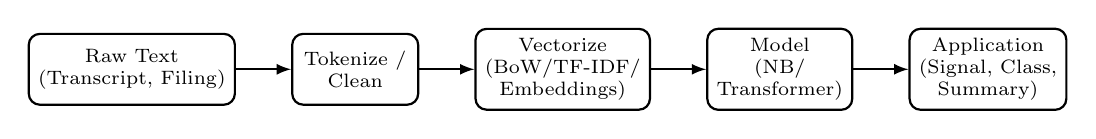
\begin{tikzpicture}[>=latex,thick,node distance=0.7cm]
        \node[draw,rounded corners,minimum width=1.7cm,minimum height=0.9cm,align=center,font=\scriptsize] (raw) {Raw Text\\(Transcript, Filing)};
        \node[draw,rounded corners,minimum width=1.6cm,minimum height=0.9cm,right=of raw,align=center,font=\scriptsize] (clean) {Tokenize /\\Clean};
        \node[draw,rounded corners,minimum width=1.9cm,minimum height=0.9cm,right=of clean,align=center,font=\scriptsize] (vec) {Vectorize\\(BoW/TF-IDF/\\Embeddings)};
        \node[draw,rounded corners,minimum width=1.8cm,minimum height=0.9cm,right=of vec,align=center,font=\scriptsize] (model) {Model\\(NB/\\Transformer)};
        \node[draw,rounded corners,minimum width=1.7cm,minimum height=0.9cm,right=of model,align=center,font=\scriptsize] (app) {Application\\(Signal, Class,\\Summary)};
        \draw[->] (raw) -- (clean);
        \draw[->] (clean) -- (vec);
        \draw[->] (vec) -- (model);
        \draw[->] (model) -- (app);
    \end{tikzpicture}
\end{lrbox}
\ifdim\wd\bookmeasuredbox<0.65\linewidth
\setlength{\bookcapwidth}{0.65\linewidth}
\else
\setlength{\bookcapwidth}{\wd\bookmeasuredbox}
\fi
\ffigbox[\bookcapwidth]{
\usebox{\bookmeasuredbox}
}{
    \caption{The text-to-application pipeline this chapter develops.}
    \label{fig:nlp_pipeline}
}
\end{figure}

\section{From Text to Numbers: Bag-of-Words and TF-IDF}\index{From Text to Numbers: Bag-of-Words and TF-IDF}
\label{sec:bow-tfidf}

Suppose an analyst has thousands of earnings-call transcripts and wants to feed them into one of Chapter 6's classifiers, every one of which expects a fixed-length numeric vector as input, not a paragraph of English text. The simplest way to turn text into a feature vector is the bag-of-words representation: fix a vocabulary of terms, and represent each document as the count of each vocabulary term it contains, discarding word order entirely. This is a drastic simplification, ``growth despite headwinds'' and ``headwinds despite growth'' produce identical vectors, but it is a surprisingly effective baseline, and it is exactly the ``word counts'' feature representation Chapter 6 anticipated for Naive Bayes text classification.

A raw count, however, overweights common words that appear in almost every document and carry little discriminating information. Term frequency-inverse document frequency (TF-IDF) corrects for this. For term $t$ in document $d$, drawn from a collection of $N$ documents,
\begin{equation*}
\text{tf-idf}(t,d) = \text{tf}(t,d) \times \ln\!\left(\frac{N}{\text{df}(t)}\right),
\end{equation*}
where $\text{tf}(t,d)$ is the raw count of $t$ in $d$ and $\text{df}(t)$ is the number of documents containing $t$ at least once. A term that appears in every document has $\text{df}(t)=N$ and therefore an idf of $\ln(1)=0$, its tf-idf weight vanishes regardless of how often it appears, while a term confined to a single document receives the largest possible idf weight.

\subsection*{A Worked Example: TF-IDF for Four Earnings-Call Sentences}\index{TF-IDF for Four Earnings-Call Sentences}

Consider four short earnings-call sentences, treated as four documents ($N=4$):

\begin{quote}
\small
$D_1$: ``revenue growth exceeded expectations this quarter''\\
$D_2$: ``management is cautious about revenue growth given the headwinds''\\
$D_3$: ``management remains confident despite the headwinds this quarter''\\
$D_4$: ``expectations were not met and revenue declined''
\end{quote}

Restricting attention to six vocabulary terms gives the term-frequency matrix in Table~\ref{tab:bow_tfidf}, alongside each term's document frequency, idf, and resulting tf-idf weight in $D_1$.

\begin{table}[htbp]
\centering
\caption{Term frequency, document frequency, idf, and TF-IDF weight in $D_1$}
\label{tab:bow_tfidf}
\begin{tabular}{lccccccc}
\toprule
Term & $D_1$ & $D_2$ & $D_3$ & $D_4$ & df & idf $=\ln(4/\text{df})$ & tf-idf in $D_1$ \\
\midrule
revenue & 1 & 1 & 0 & 1 & 3 & 0.2877 & 0.2877 \\
growth & 1 & 1 & 0 & 0 & 2 & 0.6931 & 0.6931 \\
headwinds & 0 & 1 & 1 & 0 & 2 & 0.6931 & 0.0000 \\
expectations & 1 & 0 & 0 & 1 & 2 & 0.6931 & 0.6931 \\
quarter & 1 & 0 & 1 & 0 & 2 & 0.6931 & 0.6931 \\
management & 0 & 1 & 1 & 0 & 2 & 0.6931 & 0.0000 \\
\bottomrule
\end{tabular}
\end{table}

The word ``revenue'' appears in three of the four documents, so it earns a modest idf of $\ln(4/3) \approx 0.2877$; every other listed term appears in exactly two documents, giving a larger idf of $\ln(4/2) = \ln 2 \approx 0.6931$. ``Headwinds'' and ``management'' each appear in $D_1$ zero times, so their tf-idf contribution to $D_1$'s vector is zero regardless of their idf weight, while ``growth,'' ``expectations,'' and ``quarter'' each contribute their full idf value of $0.6931$ since each occurs exactly once in $D_1$. This is the representation a downstream classifier, such as the Naive Bayes model in Section~\ref{sec:naive-bayes-text}, would receive as input in place of raw counts.

\section{Financial Sentiment Analysis and the Loughran-McDonald Dictionary}\index{Loughran-McDonald dictionary}
\label{sec:sentiment}

Suppose a trader wants to know, within seconds of an earnings call ending, whether management sounded upbeat or defensive, without waiting for an analyst to read the transcript and write a summary. The most direct way to score sentiment is a lexicon-based approach: maintain a list of positive and negative financial words, count how many of each appear in a document, and combine the counts into a tone score,
\begin{equation*}
\text{tone} = \frac{\#\text{positive words} - \#\text{negative words}}{\#\text{total words}}.
\end{equation*}
Generic sentiment lexicons, built from product reviews or general text, perform poorly in finance for exactly the reason Section~\ref{sec:text-data} raised: words like ``tax,'' ``cost,'' or ``liability'' read as negative in everyday English but are routine, neutral vocabulary in a financial filing. The Loughran-McDonald dictionary, developed specifically from 10-K filings, addresses this by classifying words into finance-specific categories (positive, negative, uncertainty, litigious, and others) based on how they actually function in financial disclosure.

\subsection*{A Worked Example: Scoring Two Earnings-Call Transcripts}\index{Scoring Two Earnings-Call Transcripts}

Using a small subset of real Loughran-McDonald positive words (\{strong, growth, exceeded, confident, improved\}) and negative words (\{cautious, headwinds, decline, declined, weak, concern, concerns\}), consider two short transcripts:

\begin{quote}
\small
Transcript A: ``revenue growth was strong this quarter and results exceeded expectations across every segment we remain confident heading into next year''\\
Transcript B: ``management is cautious about headwinds and results declined modestly we have some concerns about demand next quarter''
\end{quote}

Transcript A contains 20 words, of which 4 (growth, strong, exceeded, confident) are positive and none are negative, giving a tone score of $(4-0)/20 = 0.20$. Transcript B contains 17 words, of which none are positive and 4 (cautious, headwinds, declined, concerns) are negative, giving a tone score of $(0-4)/17 \approx -0.2353$. These two scores, one clearly positive and one clearly negative, are exactly the kind of feature that feeds directly into the event-driven trading signal developed next.

\section{A Worked Example: An Event-Driven Sentiment Trading Signal}\index{Event-Driven Sentiment Trading Signal}
\label{sec:event-driven-signal}

Chapter 11 emphasized that extracting a sentiment score from an earnings call is only half of an event-driven strategy: the signal must still be evaluated the way any trading strategy is evaluated, and eventually converted into an executed position, which is Chapter 11's concern, not this chapter's. This section stops at the first half, generating and evaluating the signal itself.

Suppose eight earnings-call events produce the tone scores and next-day stock returns in Table~\ref{tab:event_driven_signal}. A simple trading rule takes a long position when tone is positive and a short position when tone is negative, so the strategy's return on each event is $\text{sign}(\text{tone}) \times \text{return}$.

\begin{table}[htbp]
\centering
\begin{lrbox}{\bookmeasuredbox}
\begin{tabular}{lccccc}
\toprule
Event & Tone score & Next-day return (\%) & Signal & Strategy return (\%) & Correct? \\
\midrule
1 & $+0.15$ & $+1.2$ & Long & $+1.2$ & Yes \\
2 & $-0.10$ & $-0.8$ & Short & $+0.8$ & Yes \\
3 & $+0.08$ & $+0.3$ & Long & $+0.3$ & Yes \\
4 & $-0.05$ & $+0.4$ & Short & $-0.4$ & No \\
5 & $+0.20$ & $+2.1$ & Long & $+2.1$ & Yes \\
6 & $-0.18$ & $-1.5$ & Short & $+1.5$ & Yes \\
7 & $+0.02$ & $-0.2$ & Long & $-0.2$ & No \\
8 & $-0.12$ & $-0.9$ & Short & $+0.9$ & Yes \\
\bottomrule
\end{tabular}
\end{lrbox}
\ifdim\wd\bookmeasuredbox<0.65\linewidth
\setlength{\bookcapwidth}{0.65\linewidth}
\else
\setlength{\bookcapwidth}{\wd\bookmeasuredbox}
\fi
\ttabbox[\bookcapwidth]{
\usebox{\bookmeasuredbox}
}{
\caption{Eight earnings-call events: tone score, next-day return, signal, and strategy return}
\label{tab:event_driven_signal}
}
\end{table}

The strategy is correct, meaning the sign of its position matches the sign of the subsequent return, in 6 of 8 events, a 75\% hit rate. Events 4 and 7 are misses: in event 4, mildly negative tone was followed by a small positive return, and in event 7, mildly positive tone was followed by a small negative return, both events where the tone score was close to zero and therefore only weakly informative, a reminder that a sentiment signal is genuinely noisy, not a deterministic predictor. Comparing the two strategies (Sharpe-like ratio: mean divided by standard deviation, with no annualization applied here),
\begin{align*}
\text{Signal-driven strategy:} &\quad \text{mean} = 0.775\%, \ \text{std} = 0.8481\%, \ \text{Sharpe-like} = 0.9138, \\
\text{Buy-and-hold:} &\quad \text{mean} = 0.075\%, \ \text{std} = 1.1829\%, \ \text{Sharpe-like} = 0.0634.
\end{align*} The signal adds real value on this small sample, both a higher average return and a more consistent one, even though it is wrong nearly a quarter of the time. Turning this signal into an actual executed position, at the right size and without excessive market impact\index{market impact}, is exactly the execution problem Chapter 11 developed in detail.

The tone score above is a text-based sentiment measure, extracted from language rather than prices, which is worth placing alongside a second, price-based sentiment measure this book has already introduced: the CBOE Volatility Index (VIX)\index{CBOE Volatility Index (VIX)} from Chapter 5, often called the market's ``fear gauge,'' which aggregates option prices into a single, forward-looking measure of expected market-wide volatility without reading a single word of text. The two measures are complementary rather than redundant: a text-based tone score like the one above can capture sentiment specific to a single company's earnings call, information a broad market index like VIX cannot see at all, while VIX can move sharply in response to macroeconomic or geopolitical developments that never mention any single company by name and that a firm-specific sentiment model was never trained to detect. A more sophisticated event-driven strategy often conditions on both at once: using VIX as a market-wide risk-regime signal, exactly as Chapter 11 describes, alongside a firm-specific, text-derived tone score like the one developed in this section, since a positive earnings-call tone score is a genuinely different trading proposition depending on whether it arrives during a calm market or one already gripped by elevated, VIX-signaled uncertainty.

\section{Naive Bayes and Document Classification}\index{Naive Bayes and Document Classification}
\label{sec:naive-bayes-text}

Suppose a compliance team needs to sort thousands of sentences drawn from a 10-K's risk-factors section into ``Credit Risk'' or ``Market Risk'' categories, a task too large to do by hand every filing season but too nuanced for a simple keyword rule to get right on its own. Chapter 6 introduced Naive Bayes as a generative classifier that estimates
$$\Pr(y=k \mid x_1,\ldots,x_p) \propto \Pr(y=k)\prod_{j=1}^p \Pr(x_j \mid y=k)$$
and noted its particular suitability for text, where features are word counts and the conditional-independence assumption, while not literally true, distorts the result less than it might for correlated financial ratios. This section applies that model to exactly this document classification task, using only the counts of six vocabulary words (default, borrower, counterparty, volatility, rate, currency).

Table~\ref{tab:nb_training_sentences} shows the six training sentences verbatim, three representative of each class, each written in the same style as an actual 10-K risk-factors disclosure.

\begin{table}[htbp]
\centering
\caption{Training sentences for the 10-K risk-factor Naive Bayes classifier}
\label{tab:nb_training_sentences}
\begin{tabular}{p{10cm}l}
\toprule
Sentence & Label \\
\midrule
``A default by a major borrower or counterparty could trigger a chain of default across our loan portfolio.'' & Credit Risk \\
``Our borrower base includes several highly leveraged parties, and a default by any significant borrower could impair our credit portfolio.'' & Credit Risk \\
``We are exposed to counterparty risk if a significant counterparty were to default on its obligations under our agreements.'' & Credit Risk \\
``Significant volatility in interest rate markets, combined with broader market volatility, could adversely affect the value of our trading positions.'' & Market Risk \\
``Changes in the benchmark rate or the market rate environment, combined with volatility in trading conditions, could affect our net interest income.'' & Market Risk \\
``Fluctuations in the currency exchange market and adverse currency movements, together with changes in the base lending rate, could reduce our reported earnings.'' & Market Risk \\
\bottomrule
\end{tabular}
\end{table}

Counting occurrences of the six vocabulary words in each sentence, and applying Chapter 6's Section 6.16 Laplace (add-one) smoothing correction, gives the estimated word probabilities
\begin{align*}
\Pr(\text{default}\mid\text{Credit}) &= 0.3125, \\
\Pr(\text{borrower}\mid\text{Credit}) = \Pr(\text{counterparty}\mid\text{Credit}) &= 0.25, \\
\Pr(\text{volatility}\mid\text{Credit}) = \Pr(\text{rate}\mid\text{Credit}) = \Pr(\text{currency}\mid\text{Credit}) &= 0.0625, \\[4pt]
\Pr(\text{rate}\mid\text{Market}) &= 0.3333, \\
\Pr(\text{volatility}\mid\text{Market}) &= 0.2667, \\
\Pr(\text{currency}\mid\text{Market}) &= 0.20, \\
\Pr(\text{default}\mid\text{Market}) = \Pr(\text{borrower}\mid\text{Market}) = \Pr(\text{counterparty}\mid\text{Market}) &= 0.0667,
\end{align*}
reflecting each class's training vocabulary.

\subsection*{A Worked Example: Classifying an Ambiguous Sentence by Hand}\index{Classifying an Ambiguous Sentence by Hand}

Consider the held-out test sentence ``A default by a key counterparty during a period of heightened market volatility could be exacerbated by continued volatility in broader financial markets,'' with word counts (default: 1, counterparty: 1, volatility: 2, all others: 0), a genuinely ambiguous case that mentions both a credit-risk term and, twice, a market-risk term. With equal class priors $\Pr(\text{Credit}) = \Pr(\text{Market}) = 0.5$, the (unnormalized) class scores are
\begin{align*}
\text{score}(\text{Credit}) &= 0.5 \times 0.3125^1 \times 0.25^1 \times 0.0625^2 = 0.00015259, \\
\text{score}(\text{Market}) &= 0.5 \times 0.0667^1 \times 0.0667^1 \times 0.2667^2 = 0.00015802.
\end{align*}
Normalizing gives $\Pr(\text{Credit}\mid\text{doc}) \approx 0.4912$ and $\Pr(\text{Market}\mid\text{doc}) \approx 0.5088$: the model predicts Market Risk, narrowly and incorrectly, since this sentence's true label is Credit Risk. This is exactly the kind of near-toss-up case where the independence assumption's imprecision matters most, the two repeated ``volatility'' mentions tip a genuinely mixed-signal sentence to the wrong side by less than two percentage points of posterior probability.

Applying the same model to a test set of six sentences (three of each true class) produces the confusion matrix\index{confusion matrix} in Table~\ref{tab:nb_confusion}.

\begin{table}[htbp]
\centering
\caption{Confusion matrix for the 10-K risk-factor Naive Bayes classifier (positive class: Credit Risk)}
\label{tab:nb_confusion}
\begin{tabular}{lcc}
\toprule
 & Predicted Credit & Predicted Market \\
\midrule
Actual Credit & 2 (TP) & 1 (FN) \\
Actual Market & 0 (FP) & 3 (TN) \\
\bottomrule
\end{tabular}
\end{table}

Precision is $2/2 = 1.00$, recall is $2/3 \approx 0.6667$, and $F_1 \approx 0.80$: every sentence the model labeled Credit Risk really was Credit Risk, but it missed one genuine Credit Risk sentence, the ambiguous one worked through above, by classifying it as Market Risk instead.

\section{Word Embeddings: From Sparse Counts to Dense Vectors}\index{Word Embeddings: From Sparse Counts to Dense Vectors}
\label{sec:embeddings}

Bag-of-words and TF-IDF vectors are sparse and high-dimensional: with a vocabulary of tens of thousands of words, most entries in any document's 
vector are zero, and the representation has no notion that ``stock'' and ``equity'' are related concepts while ``stock'' and ``bond'' are not, every 
distinct word is just a separate, unrelated dimension. An embedding\index{Embedding} is exactly this: a fixed-length, continuous-valued vector standing in for a discrete object, here a word, chosen so that geometric closeness in the vector space reflects semantic closeness in meaning. Word embedding methods (Word2Vec and GloVe are the classical examples) learn such a dense,
low-dimensional vector for each word from patterns of co-occurrence in a large text corpus, such that words used in similar contexts end up with similar
vectors. Cosine similarity,
$$\cos(u,v) = \frac{u \cdot v}{\|u\|\,\|v\|}$$ 
is the standard way to measure how similar two embedding vectors are.

\subsection*{A Worked Example: Cosine Similarity of Toy Embeddings}\index{Cosine Similarity of Toy Embeddings}

To illustrate the geometric idea without training an actual embedding model, assign six financial terms small hand-chosen two-dimensional vectors:
\begin{align*}
\text{stock} &= (0.90, 0.20), & \text{equity} &= (0.85, 0.25), \\
\text{bond} &= (0.10, 0.90), & \text{debt} &= (0.15, 0.85), \\
\text{bullish} &= (0.80, -0.30), & \text{bearish} &= (-0.75, -0.35).
\end{align*}
Computing cosine similarity between related pairs gives $\cos(\text{stock}, \text{equity}) \approx 0.9977$ and $\cos(\text{bond}, \text{debt}) \approx 0.9980$, both close to 1, reflecting that these vectors point in nearly the same direction. Unrelated or opposed pairs behave very differently: $\cos(\text{stock}, \text{bond}) \approx 0.3234$ is only weakly similar, and $\cos(\text{bullish}, \text{bearish}) \approx -0.7000$ is strongly negative, capturing that the two terms are near-opposites. In a real embedding trained on financial text, this same geometric structure, synonyms and related concepts clustering together, opposites pointing in different directions, emerges from word co-occurrence patterns alone, without ever being told what any word means.

A second, even more striking property of well-trained embeddings is that vector \emph{arithmetic} on these representations can capture relationships between words, not just similarity, and this toy example was constructed so that the classic ``analogy'' relation holds exactly. Computing $\text{stock} - \text{equity} + \text{bond}$,
\begin{equation*}
(0.90, 0.20) - (0.85, 0.25) + (0.10, 0.90) = (0.15, 0.85) = \text{debt},
\end{equation*}
reproduces the debt vector exactly, because stock and equity, and separately bond and debt, were placed as near-synonym pairs displaced from one another by the identical offset, $(0.05, -0.05)$. In a real, trained embedding space, this same kind of arithmetic famously (if imperfectly) captures relationships like ``king $-$ man $+$ woman $\approx$ queen,'' and in a financial embedding space, an analogous relationship might hold between a company and its industry-standard debt instrument, or between a country and its currency, allowing an analyst to query the embedding space with relationships rather than only single-word similarity. Real embeddings only approximate this property, and the approximation is noticeably weaker for rarer or more abstract financial terms than for common, concrete ones, but the toy example here isolates the geometric idea cleanly before it gets obscured by the noise of a real, high-dimensional trained model.

\section{Attention and the Transformer Architecture}\index{Attention and the Transformer Architecture}
\label{sec:attention-transformers}

Embeddings give each word a fixed vector regardless of context, but the same word can mean different things in different sentences (``the Fed will likely raise rates'' versus ``the flood raised water levels''). Transformer models address this with a self-attention mechanism. Each token's embedding $x$ is linearly projected, using three weight matrices $W^Q$, $W^K$, $W^V$ that are learned during training and shared across every token in the sequence, into a query vector $Q=xW^Q$, a key vector $K=xW^K$, and a value vector $V=xW^V$; a token does not ``produce'' these vectors from nowhere, it is simply the same embedding viewed through three different learned lenses. Intuitively, a token's query asks ``what am I looking for,'' its key advertises ``what I have to offer if some other token is looking for this,'' and its value is the actual information it contributes once attention has decided to focus on it, a search query, an index entry, and a payload, respectively. A token's contextual representation is then a weighted combination of every token's value vector, with weights determined by how well each token's key matches the query,
\begin{equation*}
\text{Attention}(Q,K,V) = \text{softmax}\!\left(\frac{QK^\top}{\sqrt{d_k}}\right) V, \qquad \text{softmax}(z)_i = \frac{e^{z_i}}{\sum_j e^{z_j}},
\end{equation*}
where $d_k$ is the dimension of the key vectors, included to keep the dot products from growing too large as $d_k$ increases, and softmax\index{softmax} rescales a vector of raw scores into positive weights that sum to exactly one, so the weighted combination of value vectors that follows is a genuine, interpretable average rather than an arbitrary weighted sum. This single mechanism, applied across many layers and attention ``heads,'' is the core computational building block inside BERT, GPT, and every other modern transformer-based language model. Figure~\ref{fig:qkv_architecture} lays out this computation as a diagram, the same three-projection, one-combination structure every attention layer repeats.

\begin{figure}[htbp]
\centering
\begin{lrbox}{\bookmeasuredbox}
    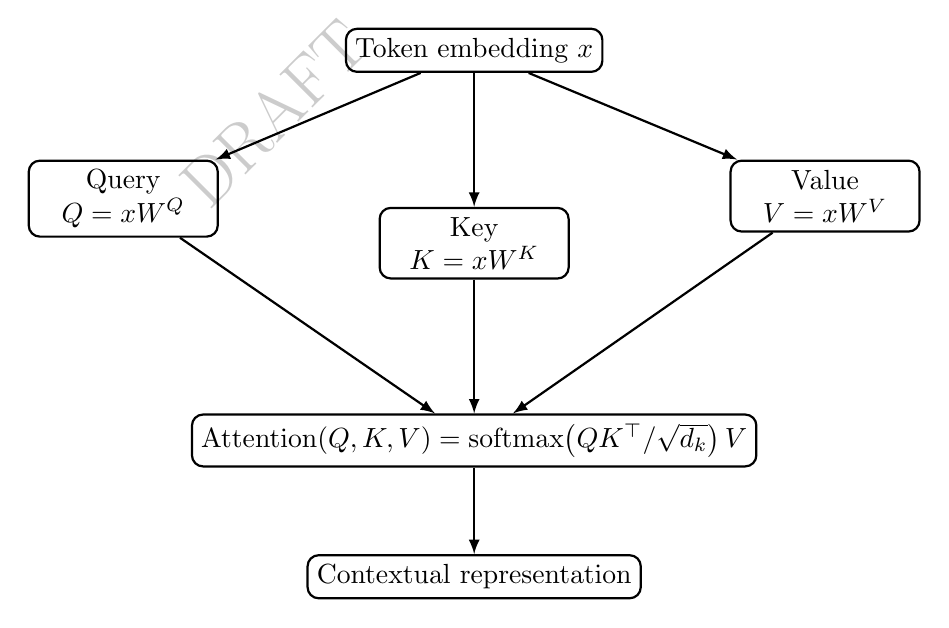
\begin{tikzpicture}[>=latex,thick,node distance=1.1cm and 1.6cm]
        \node[draw,rounded corners,align=center,minimum width=3.0cm] (embed) {Token embedding $x$};
        \node[draw,rounded corners,align=center,minimum width=2.4cm,below left=of embed] (q) {Query\\$Q=xW^Q$};
        \node[draw,rounded corners,align=center,minimum width=2.4cm,below=1.7cm of embed] (k) {Key\\$K=xW^K$};
        \node[draw,rounded corners,align=center,minimum width=2.4cm,below right=of embed] (v) {Value\\$V=xW^V$};
        \node[draw,rounded corners,align=center,minimum width=6.0cm,below=1.7cm of k] (attn) {$\text{Attention}(Q,K,V)=\text{softmax}\!\left(QK^\top/\sqrt{d_k}\right)V$};
        \node[draw,rounded corners,align=center,minimum width=3.4cm,below=1.1cm of attn] (out) {Contextual representation};
        \draw[->] (embed) -- (q);
        \draw[->] (embed) -- (k);
        \draw[->] (embed) -- (v);
        \draw[->] (q) -- (attn);
        \draw[->] (k) -- (attn);
        \draw[->] (v) -- (attn);
        \draw[->] (attn) -- (out);
    \end{tikzpicture}
\end{lrbox}
\ifdim\wd\bookmeasuredbox<0.65\linewidth
\setlength{\bookcapwidth}{0.65\linewidth}
\else
\setlength{\bookcapwidth}{\wd\bookmeasuredbox}
\fi
\ffigbox[\bookcapwidth]{
\usebox{\bookmeasuredbox}
}{
    \caption{The self-attention computation as a diagram.}
    \label{fig:qkv_architecture}
}
\end{figure}

\subsection*{A Worked Example: Self-Attention for a Three-Token Sentence}\index{Self-Attention for a Three-Token Sentence}

Consider the toy sentence ``stocks rallied today,'' with $d_k = 2$. Rather than training actual projection matrices $W^Q$, $W^K$, $W^V$, this example hand-chooses the resulting key and value vectors directly, standing in for whatever a trained model would have produced: $K_{\text{stocks}} = (1,0)$, $K_{\text{rallied}} = (0,1)$, $K_{\text{today}} = (1,1)$, and $V_{\text{stocks}} = (2,0)$, $V_{\text{rallied}} = (0,2)$, $V_{\text{today}} = (1,1)$. ``stocks'' and ``today'' were deliberately given the same first key component so that any query matching strongly on that component attends to both of them equally, exactly the effect this example is built to illustrate. Computing the contextual representation of ``stocks'' uses its query $Q_{\text{stocks}} = (1,0)$. The raw scores are $Q \cdot K_i / \sqrt{2}$: $0.7071$ against ``stocks,'' $0$ against ``rallied,'' and $0.7071$ against ``today,'' since ``stocks'' and ``today'' share a key component in the first dimension while ``rallied''s key is orthogonal to the query. Applying the softmax formula above to these three scores gives attention weights of $0.4011$, $0.1978$, and $0.4011$ respectively, which do sum to $1$ exactly as softmax guarantees, and the weighted sum of value vectors is
\begin{equation*}
0.4011\,(2,0) + 0.1978\,(0,2) + 0.4011\,(1,1) = (1.2033,\ 0.7967).
\end{equation*}
Figure~\ref{fig:attention_weights} draws these three attention weights directly, with edge thickness proportional to how much each token contributes. The token ``today,'' despite being a different word, contributes exactly as much to ``stocks'''s new representation as ``stocks'' contributes to itself, because their key vectors happen to align with the query, while ``rallied'' contributes far less, its value $(0,2)$ pulled in only weakly.

\begin{figure}[htbp]
\centering
\begin{lrbox}{\bookmeasuredbox}
    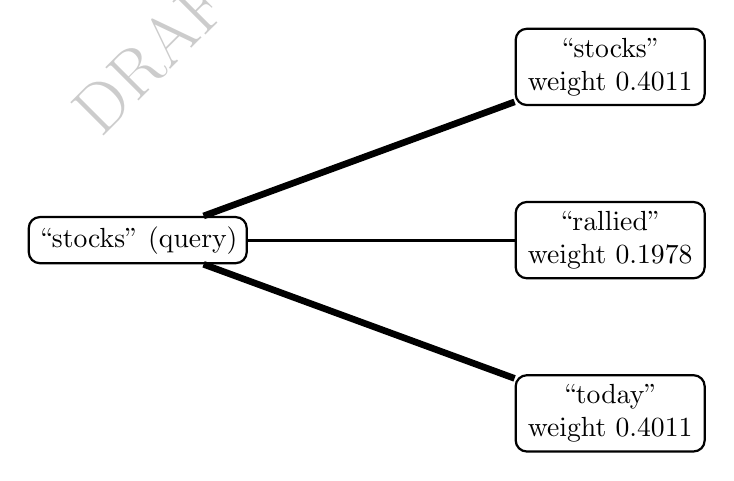
\begin{tikzpicture}[thick]
        \node[draw,rounded corners,align=center,minimum width=2.6cm] (q) at (0,0) {``stocks'' (query)};
        \node[draw,rounded corners,align=center,minimum width=2.4cm] (k1) at (6,2.2) {``stocks''\\weight $0.4011$};
        \node[draw,rounded corners,align=center,minimum width=2.4cm] (k2) at (6,0) {``rallied''\\weight $0.1978$};
        \node[draw,rounded corners,align=center,minimum width=2.4cm] (k3) at (6,-2.2) {``today''\\weight $0.4011$};
        \draw[line width=2.4pt] (q) -- (k1);
        \draw[line width=1.0pt] (q) -- (k2);
        \draw[line width=2.4pt] (q) -- (k3);
    \end{tikzpicture}
\end{lrbox}
\ifdim\wd\bookmeasuredbox<0.65\linewidth
\setlength{\bookcapwidth}{0.65\linewidth}
\else
\setlength{\bookcapwidth}{\wd\bookmeasuredbox}
\fi
\ffigbox[\bookcapwidth]{
\usebox{\bookmeasuredbox}
}{
    \caption{Self-attention weights for the query token ``stocks'' over the three-token sentence ``stocks rallied today,'' with edge thickness proportional to attention weight.}
    \label{fig:attention_weights}
}
\end{figure}

This is exactly the mechanism that lets a transformer build a contextual representation of ``raise'' that differs depending on whether nearby tokens are ``rates'' or ``water levels'': a trained $W^K$ would give ``rates'' and ``raise'' well-aligned keys in a financial context and ``water'' and ``raise'' well-aligned keys in an environmental one, precisely the way this toy example's keys were aligned by construction rather than learned from data.

\subsection*{Multi-Head Attention and Positional Encoding}\index{Multi-Head Attention and Positional Encoding}

A single attention calculation forces every token to distribute its focus according to one shared notion of relevance, but relevance in a real sentence is not one-dimensional: local grammatical structure (which word modifies which noun) and long-range dependency (which earlier passage a later reference actually points back to) are two genuinely different kinds of relationship, and a single attention pattern has no way to represent both well at once. Two refinements turn this single calculation into the mechanism actually used in practice. First, a real transformer layer computes several
attention calculations in parallel, each with its own learned $Q$, $K$, $V$ projections, called attention heads, then concatenates their outputs.
One head might learn to attend primarily to nearby tokens (useful for local syntax), another to the subject of a distant
verb (useful for long-range dependencies such as connecting a hedge's description early in a paragraph to a number reported much later),
and the model combines all of these perspectives rather than relying on a single attention pattern. Second, the attention calculation above 
treats the input as an unordered set: nothing in $Q \cdot K$ depends on token position, so ``the bank raised rates'' and ``rates 
raised the bank'' would receive identical attention weights if given identical token embeddings. Positional encoding ($PE$) fixes this by 
adding a position-dependent vector to each token's embedding before attention is computed, most commonly 
$$PE_{(pos, 2i)} = \sin\left(\frac{pos}{10000^{2i/d}}\right)$$ 
and 
$$PE_{(pos,2i+1)} = \cos\left(\frac{pos}{10000^{2i/d}}\right)$$ 
for position $pos$ and embedding dimension index $i$, so that word order, essential to meaning in any language, survives into a mechanism that would otherwise discard it entirely.

\subsection*{Encoder-Only, Decoder-Only, and Encoder-Decoder Architectures}\index{Encoder-Only, Decoder-Only, and Encoder-Decoder Architectures}

The self-attention mechanism above is the shared building block behind every transformer-based model, but different financial NLP tasks call
for arranging that block differently, and the resulting three architecture families are not interchangeable. An encoder-only model 
(BERT and its financial variant FinBERT are the standard examples) lets every token attend bidirectionally to every other token, before and after
it in the sequence, exactly the unmasked computation in the worked example above, and is trained with a masked-language-modeling objective 
(predicting a randomly hidden word from its full surrounding context in both directions). This bidirectional view makes encoder-only models well
 suited to classification and embedding tasks, such as the sentiment scoring of Section~\ref{sec:sentiment} and the document classification of 
 Section~\ref{sec:naive-bayes-text}, where the full context of a passage is available at once and the task is to produce a single label or vector, 
 not to generate new text. A decoder-only model (the GPT family, and the LLMs described throughout the rest of this chapter) instead restricts 
 each token to attending only to itself and earlier tokens, a causal mask, since it is trained to predict each next token from only what precedes 
 it, exactly the generative, one-token-at-a-time process Section~\ref{sec:llms-finance} describes. An encoder-decoder model (T5-style architectures)
 uses both: a bidirectional encoder processes the full input, and a causal decoder generates the output one token at a time while cross-attending 
 to the encoder's output, a natural fit for tasks with a clear input-to-output transformation, such as translating a filing into another language 
 or condensing a full earnings call into a short summary.

\subsubsection*{A Worked Example: How a Causal Mask Changes a Token's Representation}
Return to the ``stocks rallied today'' example, now computing the contextual representation of ``rallied'' using its own query $Q_{\text{rallied}} = (0,1)$, first with full bidirectional attention (as an encoder-only model would compute it) and then with a causal mask that hides ``today'' from ``rallied,'' since ``today'' comes after it in the sequence (as a decoder-only model would compute it). Bidirectionally, the raw scores $Q_{\text{rallied}} \cdot K_i/\sqrt{2}$ are $0$ against ``stocks,'' $0.7071$ against ``rallied,'' and $0.7071$ against ``today,'' giving softmax weights of $0.1978$, $0.4011$, and $0.4011$ and an output of
\begin{equation*}
0.1978\,(2,0) + 0.4011\,(0,2) + 0.4011\,(1,1) = (0.7967,\ 1.2033).
\end{equation*}
Under a causal mask, ``today'' is simply removed from consideration entirely, leaving only the scores against ``stocks'' ($0$) and ``rallied'' ($0.7071$); renormalizing these two alone via softmax gives weights of $0.3302$ and $0.6698$, and an output of
\begin{equation*}
0.3302\,(2,0) + 0.6698\,(0,2) = (0.6605,\ 1.3395).
\end{equation*}
The two representations of the identical word ``rallied,'' in the identical sentence, differ, $(0.7967, 1.2033)$ versus $(0.6605, 1.3395)$, purely as a consequence of architecture choice: an encoder-only model's representation of ``rallied'' is allowed to reflect that ``today'' follows it, while a decoder-only model's representation, used to predict what comes \emph{after} ``rallied,'' cannot be allowed to peek at ``today'' at all without trivializing its own training objective. This is precisely why swapping a decoder-only LLM in for a task an encoder-only model was designed for, or vice versa, is not merely a matter of using ``a big enough model'': the two produce systematically different token representations by construction, not merely by training data.

\subsection*{How These Models Are Trained, and Why They Eventually Need Retraining}\index{How These Models Are Trained, and Why They Eventually Need Retraining}

No one hand-writes the rule that lets a model correctly guess which distant word a pronoun refers to, or which number a sentence's context makes most plausible; a model this large has to learn it, and the only training signal available at the necessary scale is the text itself, with no human labels attached. None of the weight matrices in Figure~\ref{fig:qkv_architecture}, $W^Q$, $W^K$, $W^V$, or the many more inside a full transformer's feedforward and output layers, are hand-specified; every one of them is learned by ordinary gradient descent (Chapter 6's Section 6.5), applied not to a small labeled dataset but to a self-supervised objective computed directly from raw, unlabeled text at enormous scale. An encoder-only model is pretrained by masking a random fraction of tokens in each training sentence and learning to predict the missing token from its surrounding bidirectional context; a decoder-only model is pretrained on the simpler, single objective of predicting each next token from everything before it, applied repeatedly across a very large corpus of general text, exactly the causal-masked computation the worked example above just carried out by hand. This is what ``training'' actually means for a language model: no human labels the correct output token by token, the text itself supplies the training signal, which is precisely why these models can be pretrained on a vastly larger volume of data than any supervised model in this book has needed.

Pretraining is not, however, a one-time event a financial institution can complete and then ignore indefinitely. Financial language itself drifts: new instruments, regulations, tickers, and company names appear continuously, established terms occasionally acquire new meanings (a ``pandemic bond'' meant nothing before 2020), and the vocabulary a sentiment or classification model was pretrained on can gradually stop matching the vocabulary a live system actually encounters, a text-domain analogue of the concept drift Chapter 12's Section 12.17 and Chapter 16's population-stability-index discussion already raised for numeric models. Three responses are common in practice, roughly in increasing order of cost: prompting or retrieval (Section~\ref{sec:rag}) can supply current information to an otherwise-frozen model without touching its weights at all; parameter-efficient fine-tuning updates a small number of additional parameters on a modest, domain-specific dataset without repeating full pretraining; and continued pretraining resumes the original self-supervised objective on fresh text, updating the model's weights more thoroughly at proportionally higher computational cost. Which response is appropriate depends on whether the problem is a knowledge gap (the model simply lacks a recent fact, best fixed by retrieval) or a genuine shift in how language itself is used (better fixed by continued pretraining or fine-tuning), a diagnosis that itself requires the same kind of ongoing monitoring Chapter 16's model-governance discussion already established for every other model in this book.

\section{Large Language Models in Finance: Capabilities, Generative Modeling, and Limits}\index{Large Language Models in Finance: Capabilities, Generative Modeling, and Limits}
\label{sec:llms-finance}

Suppose an analyst is handed a hundred-page merger filing an hour before a decision is due, or a portfolio manager wants a plain-English answer to a specific question buried somewhere inside it, tasks none of this chapter's classification or scoring tools, built to output a single label or score, can actually perform. Chapter 6 noted that large language models are far more elaborate examples of the same generative-modeling principle behind Naive Bayes: both learn a probability distribution, Naive Bayes over word counts given a class, an LLM over the next token given all preceding tokens, and both can be used generatively, Naive Bayes to characterize what a document of a given class looks like, an LLM to produce entire new documents. An LLM is, mechanically, a very large stack of the self-attention layers developed in Section~\ref{sec:attention-transformers}, trained on enormous volumes of text to predict the next token, then further adapted (through instruction tuning and related techniques) to follow natural-language prompts.

In finance, this generative capability supports tasks well beyond the classification and scoring problems earlier sections addressed: summarizing a lengthy earnings call into a short brief, extracting a structured table of figures from an unstructured filing, drafting a first pass at a research note, or answering a natural-language question about a specific document. These are qualitatively different tasks from the fixed-output classification and scoring problems this book has otherwise emphasized, and they come with a correspondingly different failure mode: hallucination\index{Hallucination}, an LLM's tendency to generate fluent, confident-sounding text that is factually wrong, a specific number invented rather than retrieved, a filing detail misattributed, a summary that omits a covenant violation buried in a footnote. A classification model's failure mode is a wrong label with a computable error rate; an LLM's characteristic failure mode is a wrong but plausible-sounding answer, which is harder to detect automatically and more dangerous in a domain where a single invented figure in a research note or a summarized covenant can be individually consequential. The next four sections develop, in turn, the leading mitigation for hallucination (retrieval-augmented generation), how to instruct a generative model effectively (prompting), a second, distinct use of generative modeling that has nothing to do with text (synthetic data generation), and how a financial institution governs all of this in practice.

\subsection*{Beyond Text: Code Generation and Multimodal Applications}\index{Beyond Text: Code Generation and Multimodal Applications}

Two further capabilities extend an LLM's usefulness beyond the purely text-in, text-out tasks described so far. Code generation applies the same next-token prediction principle to programming languages rather than natural language: an analyst can describe a desired calculation in plain English, for example, ``load this CSV of daily returns and compute the annualized Sharpe ratio\index{Sharpe ratio} and maximum drawdown,'' and receive working Python code implementing it, directly extending the pandas- and NumPy-based analysis this book has built since Chapter 2, though the generated code still needs the same scrutiny any code does before it runs against real portfolio data, since a subtly wrong annualization factor or an off-by-one window is a bug like any other, not a hallucination in the text sense, but no less consequential. Multimodal models extend the same architecture to inputs beyond plain text, reading a scanned PDF page, a chart embedded in an investor presentation, or a table image directly, and answering questions or extracting figures from it without a separate, brittle optical-character-recognition step, which matters in practice since a great deal of financial disclosure (annual report exhibits, scanned older filings, chart-heavy investor decks) is not available as clean machine-readable text to begin with.

\section{Retrieval-Augmented Generation: A Worked Example}\index{Retrieval-Augmented Generation: A Worked Example}
\label{sec:rag}

Retrieval-augmented generation (RAG) is the most widely deployed mitigation for hallucination in financial applications. Rather than relying solely on facts an LLM absorbed during training, potentially outdated, generic, or simply never seen, a RAG system first retrieves the most relevant passages from a trusted, current document collection (a bank's own filings, policy manuals, or licensed research), then conditions the model's generated answer on those specific retrieved passages. This converts an open-ended generation task into something closer to a closed-book comprehension task: the model is asked to answer using the retrieved text, not to recall facts unaided, and its output can be traced back to a specific source passage for verification, exactly what an auditor or compliance reviewer needs.

The retrieval step is a direct application of Section~\ref{sec:embeddings}'s embedding geometry: embed the user's query and every candidate document in the same vector space, then rank documents by cosine similarity to the query and pass the top-ranked passages to the generative model.

\subsection*{A Worked Example: Retrieving the Right Passage from a Toy Knowledge Base}\index{Retrieving the Right Passage from a Toy Knowledge Base}

Consider a knowledge base of four short passages about two companies, embedded using the same hand-illustrative three-dimensional scheme as before, dimensions loosely representing revenue-topic, leverage-topic, and other-company-topic, shown in Table~\ref{tab:rag_kb}.

\begin{table}[htbp]
\centering
\caption{Toy knowledge base for the retrieval-augmented generation worked example}
\label{tab:rag_kb}
\begin{tabular}{lp{7.5cm}l}
\toprule
Document & Passage & Embedding \\
\midrule
Doc1 & ``Company X reported Q3 revenue of \$420 million, up 8\% year over year.'' & $(0.90, 0.10, 0.00)$ \\
Doc2 & ``Company X's debt-to-equity ratio increased to 1.8 in Q3.'' & $(0.10, 0.90, 0.00)$ \\
Doc3 & ``Company Y announced a new product launch in Q4.'' & $(0.00, 0.00, 0.90)$ \\
Doc4 & ``Company X's Q3 net margin improved to 12.5\% from 10.1\%.'' & $(0.60, 0.50, 0.00)$ \\
\bottomrule
\end{tabular}
\end{table}

A user asks, ``What was Company X's revenue in Q3?'', embedded as $(0.95, 0.05, 0.00)$.

Computing cosine similarity between the query and each document gives
\begin{align*}
\cos(\text{query}, \text{Doc1}) &\approx 0.9983, \\
\cos(\text{query}, \text{Doc4}) &\approx 0.8008, \\
\cos(\text{query}, \text{Doc2}) &\approx 0.1625, \\
\cos(\text{query}, \text{Doc3}) &= 0.0000.
\end{align*}
Doc1 is retrieved as the top match by a wide margin, and only Doc1 (or, at a higher retrieval count, Doc1 and Doc4) would be passed to the generative model. The model then answers using Doc1's actual text, producing ``Company X's Q3 revenue was \$420 million, up 8\% year over year,'' grounded in a retrieved, verifiable source, rather than a plausible-sounding figure invented from the model's training data alone. Note that Doc2 and Doc3, despite both mentioning Company X or a similar business topic, are correctly ranked far below Doc1 and Doc4, since neither actually answers a revenue question, exactly the discrimination a well-behaved retrieval step needs to make.

\subsection*{Evaluating a RAG System: Precision@k and a Faithfulness Score}\index{Evaluating a RAG System}

Retrieving \emph{a} document is not the same as retrieving the \emph{right} document, and a production RAG system needs a quantitative way to check both the retrieval step and the generation step separately, rather than only spot-checking final answers by hand. Precision@k measures the retrieval step alone: of the top $k$ retrieved documents, what fraction are actually relevant to the query? For the revenue question above, only Doc1 genuinely answers it; Doc4 (net margin) and Doc2 (leverage) are topically related to Company X but do not answer \emph{this} question. Ranking documents by the cosine similarities already computed (Doc1, then Doc4, then Doc2, then Doc3),
\begin{equation*}
\text{Precision@1} = \frac{1}{1} = 100\%, \qquad \text{Precision@2} = \frac{1}{2} = 50\%, \qquad \text{Precision@3} = \frac{1}{3} \approx 33.3\%,
\end{equation*}
since only one of the top-1, one of the top-2, and one of the top-3 retrieved documents is actually relevant. This is a direct, quantitative reason to keep $k$ small and the similarity threshold strict: retrieving more documents does not just add noise, it mechanically dilutes precision, which matters because every additional, non-relevant passage passed to the generative model is an additional opportunity for it to draw on irrelevant context when composing its answer.

A second, distinct check addresses the generation step: given that the right passage was retrieved, did the model's generated answer actually stick to it? A faithfulness score compares the generated answer's own embedding to the retrieved source passage's embedding, using the same cosine-similarity geometry as retrieval itself. The grounded answer from above, ``Company X's Q3 revenue was \$420 million, up 8\% year over year,'' embeds essentially identically to Doc1, at $(0.89, 0.12, 0.00)$, giving
\begin{equation*}
\text{Faithfulness} = \cos\big((0.89, 0.12, 0.00),\ \text{Doc1}\big) \approx 0.9997,
\end{equation*}
close to a perfect match, since the answer is simply restating Doc1's content. Contrast this with a hallucinated alternative answer that invents an unrelated leverage-related claim never actually stated in Doc1, embedding instead at $(0.30, 0.85, 0.00)$, closer to Doc2's topic than Doc1's:
\begin{equation*}
\text{Faithfulness} = \cos\big((0.30, 0.85, 0.00),\ \text{Doc1}\big) \approx 0.4349,
\end{equation*}
far below the grounded answer's score. A production system can use exactly this kind of threshold, flagging any generated answer whose faithfulness score against its retrieved source falls below, say, $0.85$, for automatic rejection or human review, giving the ``sample many outputs and check them against source documents for factual grounding'' validation practice Section~\ref{sec:genai-governance} calls for a concrete, computable form rather than only a qualitative principle.

\section{Prompting Strategies for Financial Tasks}\index{Prompting Strategies for Financial Tasks}
\label{sec:prompting}

How a task is phrased to a generative model, its prompt, materially affects output quality, and three prompting strategies recur across financial applications. Zero-shot prompting\index{Zero-Shot Prompting} simply states the task: ``Classify the sentiment of the following earnings-call excerpt as positive, negative, or neutral: \emph{[excerpt]}.'' This works reasonably well for common, well-defined tasks but can be inconsistent for tasks with domain-specific conventions the model has not reliably learned, exactly the kind of finance-specific vocabulary issue Section~\ref{sec:text-data} raised.

Few-shot prompting\index{Few-Shot Prompting} adds a small number of worked examples directly in the prompt before the actual task, showing the model the specific labeling convention wanted: two or three (excerpt, label) pairs, drawn perhaps from Section~\ref{sec:sentiment}'s transcripts, followed by a new, unlabeled excerpt to classify. This is analogous to Chapter 6's supervised learning setup, except the ``training'' happens entirely within a single prompt, with no weight updates to the model at all, and the ``training set'' can be as small as two or three examples.

Chain-of-thought prompting\index{Chain-of-Thought Prompting} asks the model to reason step by step before producing a final answer, rather than jumping directly to a conclusion, for example: ``First identify the reported revenue figure and the prior-year figure, then compute the percentage change, then state whether this represents an acceleration or deceleration relative to the previous quarter's growth rate, showing each step.'' For multi-step numerical tasks, computing a financial ratio from figures buried in a paragraph, or reconciling two differently defined metrics, this measurably reduces errors relative to asking for the final number directly, since it forces the model's intermediate steps into the output where they can be checked, in much the same spirit as this book's insistence, established in Chapter 7 and followed throughout, on showing every intermediate step of a calculation rather than only its final result.

\section{Generative Models for Synthetic Financial Data}\index{Generative Models for Synthetic Financial Data}
\label{sec:generative-synthetic}

A second, quite different application of generative modeling has nothing to do with text: generating entirely new, synthetic numerical data, additional stress-test scenarios, synthetic order-book sequences, or extra examples of a rare event class, that resembles real data closely enough to be useful for training or testing other models. Two architectures dominate this use case.

A generative adversarial network\index{generative adversarial network (GAN)} (GAN) pits two neural networks against each other: a generator $G$ that maps random noise $z$ to synthetic samples $G(z)$, and a discriminator $D$ that tries to distinguish real samples from generated ones, trained jointly via
\begin{equation*}
\min_G \max_D \; \mathbb{E}_{x}\!\left[\log D(x)\right] + \mathbb{E}_{z}\!\left[\log\big(1 - D(G(z))\big)\right].
\end{equation*}
As training proceeds, the generator improves at fooling the discriminator and the discriminator improves at catching it, and at convergence the generator produces samples the discriminator can no longer reliably distinguish from real data. In finance, this has been applied to augmenting a fraud detection model's minority class, extending Chapter 13's discussion of resampling techniques such as SMOTE\index{SMOTE} with entirely synthetic, rather than interpolated, minority-class examples, and to generating synthetic limit-order-book sequences for backtesting execution algorithms without exposing real client order flow.

The companion notebook evaluates this minimax game concretely, reusing Chapter 13's fraud-scoring data: a fixed, illustrative discriminator $D(x) = \sigma(2.0x - 5.0)$ assigns transaction 1's real fraud amount $z$-score of $3.1$ a probability of being real of $D(x_{\text{real}}) = 0.7685$, fairly confident. An early-training generator, still producing unrealistic samples close to a typical legitimate transaction's scale, might output $G(z) = 1.0$, which the discriminator correctly flags as almost certainly fake, $D(G(z)) = 0.0474$, a wide gap of $0.7211$ from $D(x_{\text{real}})$. A later-training generator that has learned to produce a more realistic, fraud-scale sample, $G(z) = 2.9$, is assigned $D(G(z)) = 0.6900$, closing the gap to just $0.0786$, exactly the ``generator improves at fooling the discriminator'' dynamic described above, made concrete: the generator's loss, $-\log D(G(z))$, falls from $3.0486$ at the early stage to $0.3711$ at the later stage, a direct numerical measure of how much harder the generator has become to catch.

GANs are also well known for being difficult to train in practice. Because the generator and discriminator are optimized simultaneously against each other rather than toward a single, shared objective, training can fail to converge, oscillating rather than settling into an equilibrium, or collapse into mode collapse\index{Mode Collapse}, where the generator discovers a small number of samples that reliably fool the discriminator and stops exploring the rest of the data distribution, producing synthetic fraud examples or stress scenarios that are realistic but insufficiently diverse to be useful for the very purpose, augmenting a thin dataset, they were generated for. This instability, not a limitation shared by every generative architecture, is one reason diffusion models, described next, have become the more common choice for new synthetic-data applications despite being more computationally expensive to sample from.

Diffusion models take a different approach, motivated by physical diffusion processes: a forward process gradually adds noise to real data over many steps until it becomes indistinguishable from pure noise, $x_t = \sqrt{\alpha_t}\, x_0 + \sqrt{1-\alpha_t}\,\epsilon$, where $x_0$ is the original data point, $\epsilon$ is standard-normal noise, and $\alpha_t$ decreases from near 1 (step 0, almost no noise) toward 0 (fully noised) as $t$ increases. A neural network is then trained to reverse this process, predicting and removing noise one step at a time, so that starting from pure random noise and running the learned reverse process produces an entirely new, synthetic sample resembling the original data distribution.

\subsection*{A Worked Example: One Forward Diffusion Step}\index{One Forward Diffusion Step}

Consider a toy stress-test scenario variable, a multiplier applied to a baseline loss, with baseline (undiffused) value $x_0 = 1.00$ (no stress) and a noise draw $\epsilon = 0.50$. At an early diffusion step with 
$\alpha_t = 0.80$, 
$$x_t = \sqrt{0.80}\,(1.00) + \sqrt{0.20}\,(0.50) = 1.1180.$$ 
At a later, noisier step with $\alpha_t = 0.55$, 
$$x_t = \sqrt{0.55}\,(1.00) + \sqrt{0.45}\,(0.50) = 1.0770.$$ 
As $\alpha_t$ falls from 0.80 to 0.55, the scenario value moves from 1.1180 down to 1.0770, 
drifting away from the deterministic baseline of 1.00 and toward the random noise draw of 0.50; continuing this process to $\alpha_t \to 0$ 
would carry $x_t$ all the way to $\epsilon$ itself, pure noise with no remaining trace of the original scenario. A trained diffusion model learns 
to run exactly this process in reverse, starting from noise and reconstructing a plausible, never-before-observed stress scenario, one that 
Chapter 8's stress-testing discussion could use to probe portfolio losses under conditions beyond anything in the historical sample.

\section{Governance and Risk Management for Generative AI}\index{Governance and Risk Management for Generative AI}
\label{sec:genai-governance}

Chapter 13 developed a three-lines-of-defense governance framework for fraud and compliance models; generative AI systems need the same discipline, applied to a set of risks classical, deterministic models did not raise. Three deserve particular attention. First, non-determinism: the same prompt submitted twice can produce two different outputs, which complicates traditional model validation approaches that assume a fixed model produces a fixed, reproducible output for a fixed input, and pushes validation toward statistical sampling of many outputs rather than checking a single deterministic result. Second, prompt injection: adversarial text embedded in a retrieved document, an uploaded file, or even ordinary user input can attempt to hijack a generative system's behavior, for example a malicious instruction hidden inside a retrieved filing that reads, to the model, as an instruction to ignore its original task, an attack surface with no real counterpart in the classification models earlier chapters developed. Third, data leakage: a RAG system with access to sensitive internal documents can, if not carefully scoped, surface information to a user who should not see it, turning a helpful retrieval feature into an inadvertent access-control failure.

These risks change how the third line's independent validation function, introduced in Chapter 13, must operate: rather than checking a model's predictions against a fixed, labeled test set, validating a generative system requires sampling many outputs, checking them against source documents for factual grounding (exactly the kind of check Section~\ref{sec:rag}'s retrieval step is meant to support), and explicitly testing for prompt-injection and data-leakage vulnerabilities before deployment, not just at initial launch but on an ongoing basis as the underlying model, retrieved document collection, or user population changes. Regulators have generally extended existing model risk management\index{model risk management} guidance, rather than writing entirely new rules, to cover these systems, which means a generative AI deployment must satisfy the same governance expectations, documented validation, ongoing monitoring, and a clear escalation path, developed for the classical models earlier chapters covered, even though the tools available to satisfy them look different in practice.

\section{Advanced Topics: Fine-Tuning, Agents, and Domain Adaptation}\index{Advanced Topics: Fine-Tuning, Agents, and Domain Adaptation}
\label{sec:advanced-nlp}

The base LLM described in Section~\ref{sec:llms-finance}, trained only to predict the next token, is not yet the helpful, instruction-following assistant Section~\ref{sec:rag} and this chapter's case vignette describe. Four further ideas, increasingly used in financial NLP systems, close that gap.

\subsection*{Fine-Tuning and Reinforcement Learning from Human Feedback}\index{Fine-Tuning and Reinforcement Learning from Human Feedback}

A model pretrained purely to predict the next token is, left as is, an unreliable assistant: asked a direct question, it may just as easily continue writing more text in the same style as actually answer it, since nothing in next-token prediction alone teaches it to follow an instruction or to prefer a helpful, honest response over a fluent but unhelpful one. After next-token pretraining, a model is typically further trained in two stages: supervised fine-tuning on curated (prompt, ideal response) pairs,
teaching it to follow instructions rather than merely continue text, and reinforcement learning from human feedback\index{reinforcement learning from
human feedback (RLHF)} (RLHF), which uses human preference judgments between pairs of candidate outputs to train a reward model, then adjusts the LLM 
to produce outputs that reward model scores highly. The reward model itself is typically trained as a preference classifier: given two candidate 
outputs with reward scores $r_A$ and $r_B$, the Bradley-Terry model\index{Bradley-Terry Model} estimates the probability that a human would prefer output $A$ as
$$\Pr(A \succ B) = \text{sigmoid}(r_A - r_B) = \frac{1}{1+e^{-(r_A - r_B)}}.$$

\subsubsection*{A Worked Example: Reward-Model Preference Probability}
Suppose a reward model scores a well-grounded, source-accurate earnings-call summary at $r_A = 2.1$ and a fluent but subtly inaccurate alternative summary at $r_B = 0.8$. The estimated preference probability is $\text{sigmoid}(2.1 - 0.8) = \text{sigmoid}(1.3) \approx 0.7858$: the reward model favors the accurate summary about 78.6\% of the time it is compared against the inaccurate one, and RLHF training nudges the underlying LLM's outputs toward whichever behavior the reward model scores this way, in aggregate across many such comparisons.

\subsection*{Parameter-Efficient Fine-Tuning: Low-Rank Adaptation (LoRA)}\index{Low-Rank Adaptation (LoRA)}

RLHF and supervised fine-tuning both describe \emph{what} a model is trained to do after pretraining; a separate, practical question is \emph{how} that further training is actually carried out, since updating every one of a large model's weights, full fine-tuning, requires storing a full second copy of the model's parameters (the update itself) alongside the original, and repeating this for every downstream task or client is prohibitively expensive at the scale of a modern LLM. Low-Rank Adaptation (LoRA) is the most widely used solution: instead of learning a full, dense weight update $\Delta W$ for a $d\times d$ weight matrix, LoRA constrains the update to a low-rank decomposition, $\Delta W = BA$, where $B$ is $d\times r$, $A$ is $r\times d$, and the rank $r$ is chosen to be far smaller than $d$. Only $B$ and $A$ are trained; the original weight matrix $W$ is frozen entirely, and the adapted model's forward pass simply uses $W + BA$ in place of $W$.

\subsubsection*{A Worked Example: Parameter Reduction from Low-Rank Adaptation}
Consider a single $d=4{,}096$ weight matrix, a realistic dimension for one attention or feedforward projection inside a modern LLM. Full fine-tuning of this one matrix requires learning all $d^2 = 4{,}096^2 = 16{,}777{,}216$ entries of $\Delta W$. Using LoRA with rank $r=8$, the trainable parameters are instead only those of $B$ ($d \times r$) and $A$ ($r \times d$),
\begin{equation*}
2 \times d \times r = 2 \times 4{,}096 \times 8 = 65{,}536,
\end{equation*}
a reduction factor of $16{,}777{,}216 / 65{,}536 = 256\times$ for this single matrix, and a comparable reduction applies across every weight matrix LoRA is attached to throughout the model. This is precisely why LoRA has become the default way to adapt a large financial-domain model (fine-tuning a base LLM on a specific bank's internal document style, or a specific asset class's terminology) without either the storage cost of a full duplicate model per use case or the computational cost of updating billions of frozen parameters that full fine-tuning would otherwise touch: the frozen base model, potentially already quantized using this section's own quantization technique described below, can be shared across many clients or tasks, with only a small, task-specific $B$ and $A$ pair, a few tens of thousands of parameters rather than billions, stored and swapped in per use case.

\subsection*{LLM Agents and Tool Use}\index{LLM Agents and Tool Use}

Computing and cross-checking a company's P/E ratio requires looking up its current price, pulling its latest reported earnings from a filing, dividing the two, and comparing the result against a sector benchmark, a sequence of lookups and arithmetic no single LLM call, which only ever produces text in one pass, can carry out on its own. An agent extends a single-turn LLM call into a multi-step loop: the model can decide to call an external tool, a retrieval system, a calculator, a database query, or a trading API, observe the tool's result, and decide on a next action, repeating until it produces a final answer. This directly composes the retrieval mechanism of Section~\ref{sec:rag} with ordinary computation.

\subsubsection*{A Worked Example: A Three-Step Agent Computing and Cross-Checking a P/E Ratio}
Suppose an agent is asked, ``What is Company X's price-to-earnings ratio using its Q3 diluted EPS and quarter-end share price?'' The agent first calls a retrieval tool (exactly Section~\ref{sec:rag}'s mechanism) against the same kind of knowledge base, retrieving two facts: diluted EPS of \$3.15 and a quarter-end closing price of \$57.87. It then calls a calculator tool rather than attempting the arithmetic itself, computing $\text{P/E} = 57.87 / 3.15 \approx 18.37$. Delegating the arithmetic to a calculator tool, rather than having the LLM compute it directly, removes an entire category of arithmetic-hallucination risk, since a calculator's division is exact by construction, while an LLM asked to divide two numbers directly can still make an outright arithmetic error despite retrieving perfectly correct inputs.

A more robust agent does not stop once it has an answer; it takes a third step, calling a second, independent tool to cross-check the result before presenting it. Suppose the agent additionally queries a market-data vendor's own reported P/E for Company X, retrieving $19.10$. Comparing this against its own computed value,
\begin{equation*}
\text{Discrepancy} = \frac{19.10 - 18.37}{18.37} \approx 3.97\%,
\end{equation*}
exceeds a pre-set tolerance of, say, $2\%$, so rather than presenting either number as a confident final answer, the agent flags the disagreement explicitly, for example reporting both figures along with a note that they differ by more than the tolerance and that the discrepancy may reflect a timing difference (the vendor's figure may use trailing rather than diluted EPS, or a different price snapshot) worth investigating before either number is used in a client-facing report. This cross-check step costs one additional tool call but converts a single, silently-possibly-wrong number into either a confidently validated one or an explicitly flagged discrepancy, exactly the kind of independent-verification discipline Chapter 8's model-validation framework requires of a classical risk model, now applied to a single agentic tool-use chain.

\subsection*{Mixture-of-Experts: Scaling Without Proportional Compute}

Making a language model more capable usually means making it larger, but a larger dense feedforward network makes every single token more expensive to process, whether or not that token's context actually needed the model's full capacity. A mixture-of-experts\index{mixture of experts} (MoE) architecture replaces a single large feedforward network inside each transformer layer with several smaller ``expert'' networks and a router that sends each token to only a handful of them, letting total model capacity grow without a proportional increase in the compute needed per token.

\subsubsection*{A Worked Example: Sparse Activation Fraction}
Consider a MoE layer with 8 experts of 6 billion parameters each (48 billion total expert parameters) that routes each token to only its top 2 experts. Each token activates $2 \times 6 = 12$ billion of the 48 billion expert parameters, an active fraction of $12/48 = 0.25$, or 25\%: the model has the representational capacity of a 48-billion-parameter feedforward layer while each token's forward pass costs only what a 12-billion-parameter layer would.

\subsection*{Domain-Adapted Financial Language Models: BloombergGPT\index{BloombergGPT}}\index{Domain-Adapted Financial Language Models: BloombergGPT}

Section~\ref{sec:sentiment}'s Loughran-McDonald dictionary made a simple, lexicon-based version of a broader point: general-purpose tools built on general-purpose text underperform on financial language. BloombergGPT, announced by Bloomberg in 2023, applies the same principle to a full-scale LLM rather than a hand-built word list: a 50-billion-parameter model trained from scratch on a mixed corpus of over 700 billion tokens, roughly 363 billion tokens of Bloomberg's own financial data (news, filings, and other proprietary financial text spanning decades) combined with roughly 345 billion tokens of general-purpose text, with 569 billion tokens actually sampled for training. The model outperformed similarly sized general-purpose models on financial-specific benchmarks (sentiment analysis, financial named-entity recognition, and financial question answering) while remaining competitive with them on general-purpose language benchmarks, empirical confirmation, at LLM scale, of the same domain-specificity argument Section~\ref{sec:text-data} made about financial vocabulary at the very start of this chapter.

\subsection*{Quantization: Deploying a Large Model at Lower Cost}\index{Quantization: Deploying a Large Model at Lower Cost}

A financial institution that wants to run a model like BloombergGPT on its own infrastructure, rather than sending every query to an external provider's API, an important consideration given Section~\ref{sec:genai-governance}'s data-leakage concern, faces a direct memory and compute cost. Quantization reduces this cost by storing each parameter with fewer bits than the precision used during training, trading a small amount of accuracy for a large reduction in memory footprint.

\subsubsection*{A Worked Example: Memory Footprint Under Quantization}
A 50-billion-parameter model held at 16-bit precision (2 bytes per parameter) requires $50\times10^9 \times 2 = 100\times10^9$ bytes, 100 gigabytes, just to store its weights, before accounting for activations or the memory a long conversation's key-value cache consumes. Quantizing to 8-bit precision (1 byte per parameter) halves this to 50 gigabytes, and quantizing further to 4-bit precision (0.5 bytes per parameter) brings it to 25 gigabytes, a fourfold reduction from the original 16-bit footprint. This is exactly the kind of trade-off, some accuracy degradation in exchange for a model that fits on cheaper hardware and answers faster, that determines whether an institution can feasibly run a domain-adapted model like this in-house at all, rather than as a purely theoretical exercise.

\subsubsection*{A Worked Example: API Cost Versus Self-Hosting at Scale}
Quantization's payoff is easiest to see by putting a dollar figure on the alternative. Suppose an institution's financial-research assistant handles $40{,}000$ queries per day, averaging $1{,}000$ tokens per query (prompt plus response), against an external provider charging $\$0.03$ per $1{,}000$ tokens. The daily API cost is
\begin{equation*}
40{,}000 \times \frac{1{,}000}{1{,}000} \times \$0.03 = \$1{,}200, \qquad \text{or } \$1{,}200 \times 30 \approx \$36{,}000 \text{ per month.}
\end{equation*}
Running the same 4-bit-quantized 50-billion-parameter model in-house instead, on hardware processing $4{,}000$ queries per hour, requires $40{,}000/4{,}000 = 10$ hours of GPU time per day; at a cloud GPU rental rate of $\$20$ per hour, this comes to $10 \times \$20 = \$200$ per day, or $\$200 \times 30 = \$6{,}000$ per month, a sixfold reduction from the API-based cost at this query volume. This comparison is exactly why the earlier memory-footprint calculation is not merely a technical curiosity: a model that only fits in memory at 4-bit precision, on a single accessible GPU rather than a multi-GPU cluster, is precisely the model that makes the \$6,000-per-month self-hosted alternative achievable at all, and the volume at which self-hosting overtakes an API's convenience is exactly the kind of build-versus-buy calculation Section~\ref{sec:genai-governance}'s data-leakage concern makes doubly relevant, since self-hosting also keeps every query's content inside the institution's own infrastructure rather than sending it to an external provider.

\section{Disclosure Analysis: Readability and the Gunning Fog Index}\index{Disclosure Analysis: Readability and the Gunning Fog Index}
\label{sec:disclosure-analysis}

Regulators require that public disclosures be understandable to ordinary investors (the U.S. Securities and Exchange Commission's ``Plain English'' rule is one such requirement), and readability metrics give a simple, quantitative way to assess whether a given passage meets that bar. The Gunning Fog index estimates the years of formal education a reader needs to understand a passage on a first reading,
\begin{equation*}
\text{Fog} = 0.4 \left[ \frac{\text{words}}{\text{sentences}} + 100 \times \frac{\text{complex words}}{\text{words}} \right],
\end{equation*}
where a complex word is (approximately) one with three or more syllables.

\subsection*{A Worked Example: Two Disclosure Paragraphs Compared}\index{Two Disclosure Paragraphs Compared}

Consider two short passages. Paragraph A: ``The firm's sales grew this year. Profits also rose. We expect this trend to grow next year.'' This has 17 words across 3 sentences and zero complex words (every word has one or two syllables), giving $\text{Fog} = 0.4\,[(17/3) + 100(0/17)] = 2.27$. Paragraph B: ``The Company's operations are subject to numerous regulatory, competitive, and macroeconomic uncertainties. These uncertainties could materially and adversely affect anticipated profitability and operational continuity.'' This has 24 words across 2 sentences, of which 14 are complex (numerous, regulatory, competitive, macroeconomic, uncertainties, materially, adversely, anticipated, profitability, operational, continuity, and others), giving $\text{Fog} = 0.4\,[(24/2) + 100(14/24)] = 28.13$.

A Fog index above roughly 17 corresponds to a post-graduate reading level; Paragraph B's score of 28.13 is far beyond that, and while these two toy paragraphs are deliberately constructed to contrast sharply, the direction of the result matches a well-documented empirical finding: 10-K risk-factor sections and other mandatory disclosures routinely score in this same elevated range in practice, dense, technical, and long-sentence, and readability metrics like this one give compliance and research teams a simple, automatable way to flag disclosures that may not be meeting the plain-English standard regulators intend, or, for a research application, to test whether unusually low readability in a given filing is itself a predictive signal (some published research finds that harder-to-read disclosures are associated with worse subsequent firm performance, consistent with obfuscation being used strategically).

The Fog index is also useful as a diagnostic during the drafting process itself, not only after the fact. Rewriting Paragraph B in plainer language, ``Our business faces many risks from rules, competition, and the economy. These risks could hurt our profits and how well we operate,'' gives 23 words across 2 sentences with only 3 complex words (competition, economy, operate), so
\begin{equation*}
\text{Fog} = 0.4\,[(23/2) + 100(3/23)] \approx 9.82,
\end{equation*}
close to Paragraph A's toy score and nowhere near Paragraph B's original 28.13, despite covering essentially the same substantive content, the same categories of risk and the same warning about their potential effect on profitability. This is precisely the practical use case regulators intend a Plain English rule to encourage: the underlying legal and business meaning did not need to change at all to bring the Fog score down by nearly two-thirds, only the sentence structure and word choice, which is exactly why an automated readability check integrated directly into a disclosure-drafting workflow can flag an overly complex passage for simplification before it is ever filed, rather than only after a regulator or researcher measures it externally.

\section{Case Vignette: AI @ Morgan Stanley}\index{Morgan Stanley}

In September 2023, Morgan Stanley announced that AI @ Morgan Stanley Assistant, built together with OpenAI on GPT-4, was fully live for its wealth management financial advisors and support staff. The assistant is, in this chapter's terms, a retrieval-augmented generation system: it gives advisors natural-language access to the firm's ``intellectual capital,'' a collection of roughly 100,000 research reports and internal documents, retrieving the passages relevant to an advisor's question and generating an answer grounded in them, exactly the mechanism Section~\ref{sec:rag} worked through on a toy four-document example. Morgan Stanley later reported that the tool reached over 98\% adoption among advisor teams, and that the share of the firm's research content advisors could effectively find and use rose from roughly 20\% to roughly 80\%, a direct measure of the retrieval problem Section~\ref{sec:rag} illustrated at genuinely large scale rather than four toy documents.

The firm subsequently extended the same underlying models to a second, structurally different application: AI @ Morgan Stanley Debrief, which uses OpenAI's Whisper speech-to-text model together with GPT-4 to turn a client meeting recording, made only with the client's consent, into a structured summary, client notes filed automatically into the firm's customer relationship management system, and a draft follow-up email an advisor reviews and sends. This is squarely the summarization capability Section~\ref{sec:llms-finance} described, deployed on genuinely sensitive input (a recorded client conversation) rather than a public filing, which is precisely why consent, access control, and human review before anything reaches a client are treated as first-class design requirements rather than afterthoughts, the same governance discipline Section~\ref{sec:genai-governance} argued a generative AI deployment needs from the outset. A third tool, AskResearchGPT, later extended the same retrieval-augmented pattern from wealth management into the firm's institutional research business, illustrating that a well-built RAG system, once validated for one internal use case, tends to generalize to others faster than building a comparable system from scratch each time.

The case is instructive for this chapter specifically because its two headline results, near-total adoption and a fourfold increase in effective document accessibility, came not from a more powerful underlying model than any other firm could license, but from the unglamorous, chapter-spanning work this chapter has emphasized throughout: a well-curated retrieval corpus, a retrieval mechanism grounded in the same cosine-similarity geometry Section~\ref{sec:embeddings} introduced, and a governance structure, consent for Debrief's recordings, human review of drafted outputs, that made deployment at scale defensible.

\section{Challenges in Natural Language Processing in Finance}

Several challenges recur across the techniques this chapter developed, and many connect to themes from earlier chapters.

\textbf{Domain-specific vocabulary defeats generic tools.} As Section~\ref{sec:text-data} emphasized, sentiment lexicons and language models trained on general text routinely misread financial language, which is exactly why finance-specific resources like the Loughran-McDonald dictionary exist and why even a large general-purpose language model benefits from finance-specific fine-tuning or careful prompting.

\textbf{A weak signal is still noisy, not deterministic.} Section~\ref{sec:event-driven-signal}'s trading signal added real value on average, a higher mean return and a better Sharpe-like ratio than buy-and-hold, while still being wrong on two of eight events, a reminder that an NLP-derived signal is a probabilistic input to a strategy, not a certainty, exactly the same lesson Chapter 6 emphasized about model evaluation generally.

\textbf{Hallucination is a qualitatively different failure mode than misclassification.} A classifier's error rate is directly computable from a confusion matrix, as Section~\ref{sec:naive-bayes-text} demonstrated; an LLM's tendency to generate fluent, wrong answers, discussed in Section~\ref{sec:llms-finance}, has no equally clean error rate, since detecting a hallucination often requires the same domain expertise the tool was meant to save. Retrieval-augmented generation (Section~\ref{sec:rag}) mitigates this, but does not eliminate it: a model can still misread or misquote a correctly retrieved passage.

\textbf{Generative AI introduces risks classical models never raised.} Non-deterministic outputs, prompt injection, and RAG-related data leakage, all discussed in Section~\ref{sec:genai-governance}, have no real counterpart in the deterministic classification and scoring models Chapters 6 through 12 developed, and require validation approaches, statistical sampling of outputs rather than checking a single fixed prediction, that those earlier chapters' models did not need.

\textbf{Explainability and audit requirements constrain deployment.} As Chapter 16 develops further, a trading decision or disclosure classification influenced by an NLP model may need to be explained after the fact, which is more difficult for the deep, attention-based architectures of Section~\ref{sec:attention-transformers} than for the transparent, inspectable probabilities of Section~\ref{sec:naive-bayes-text}'s Naive Bayes classifier.

\textbf{Data licensing and evaluation are both harder than they look.} High-quality financial text, especially real-time news and licensed data feeds, is expensive and contractually restricted, and evaluating an NLP system's real-world performance is harder than evaluating a numerical model, since two humans often disagree about the ``correct'' sentiment or summary for a given passage, so even the ground truth used to measure accuracy is itself somewhat subjective.

\section{Key Takeaways}

Financial text must be converted into numerical features before any of this book's earlier tools apply to it, and this chapter developed that conversion end to end: bag-of-words and TF-IDF (Section~\ref{sec:bow-tfidf}) turn text into sparse count vectors, the Loughran-McDonald lexicon (Section~\ref{sec:sentiment}) turns those vectors into a finance-specific sentiment score, and word embeddings (Section~\ref{sec:embeddings}) replace sparse counts with dense vectors that capture semantic similarity geometrically. A lexicon-based sentiment score is a genuinely useful but noisy trading signal, as Section~\ref{sec:event-driven-signal} showed with a 75\% hit rate that still outperformed buy-and-hold on both average return and consistency, and generating that signal is only half the task Chapter 11 develops in full. Naive Bayes, introduced as an abstract generative classifier in Chapter 6, applies directly to document classification (Section~\ref{sec:naive-bayes-text}), including the genuinely ambiguous cases where its conditional-independence assumption's imprecision is most visible. Self-attention (Section~\ref{sec:attention-transformers}) is the mechanism that lets transformer-based models, including the large language models of Section~\ref{sec:llms-finance}, build context-dependent representations of text, and those same models' generative capability supports summarization and information extraction well beyond classification, at the cost of a qualitatively new failure mode, hallucination, that a computable error rate cannot fully capture. Retrieval-augmented generation (Section~\ref{sec:rag}) is the leading mitigation, grounding generated answers in specific, verifiable source passages, while prompting strategy (Section~\ref{sec:prompting}), zero-shot, few-shot, or chain-of-thought, shapes how 
reliably a generative model performs a given task without any change to the model itself. Generative modeling extends well beyond text: GANs and 
diffusion models (Section~\ref{sec:generative-synthetic}) generate entirely synthetic numerical data, additional minority-class fraud examples or 
stress-test scenarios beyond the historical sample, by learning to reverse a noising process or to fool an adversarially trained discriminator. 
All of this requires governance (Section~\ref{sec:genai-governance}) that extends Chapter 13's three-lines-of-defense framework to risks, 
non-determinism, prompt injection, data leakage, that classical, deterministic models never presented. Section~\ref{sec:advanced-nlp} went one 
level deeper still: RLHF's reward modeling turns human preferences into a trainable signal, agents compose retrieval with actual computation 
(and should delegate arithmetic to a calculator tool rather than trust an LLM's own division), mixture-of-experts architectures decouple model 
capacity from per-token compute cost, and BloombergGPT demonstrates the Loughran-McDonald dictionary's domain-specificity argument holding at full
 LLM scale. Finally, readability metrics like the Gunning Fog index (Section~\ref{sec:disclosure-analysis}) turn a regulatory concern, whether disclosure
  is genuinely understandable, into a simple, automatable measurement.

\section{Suggested Exercises}

\begin{enumerate}
    \item Using Table~\ref{tab:bow_tfidf}'s method, compute the idf and tf-idf weight (in $D_2$) for a seventh term, ``confident,'' which appears once in $D_3$ only, and explain why its idf is the largest of any term considered so far.
    \item Extend Table~\ref{tab:bow_tfidf}'s corpus with a fifth document, $D_5$: ``revenue and growth both declined this quarter,'' and recompute the document frequency and idf for ``revenue,'' ``growth,'' and ``quarter.''
    \item Using Section~\ref{sec:sentiment}'s method and word lists, compute the tone score for the sentence ``results were weak and management remains cautious about the coming quarter despite improved margins.''
    \item Using Table~\ref{tab:event_driven_signal}'s method, add a ninth event with tone score $+0.11$ and next-day return $-0.6\%$, and recompute the strategy's hit rate, mean return, and Sharpe-like ratio.
    \item Explain, using events 4 and 7 in Table~\ref{tab:event_driven_signal}, why a tone score close to zero is a weaker signal than one far from zero, and propose a modification to the trading rule that would account for this (for example, only trading when $|\text{tone}| $ exceeds some threshold).
    \item Using Section~\ref{sec:naive-bayes-text}'s fitted word probabilities, classify a new sentence with word counts (default: 0, borrower: 1, counterparty: 1, volatility: 0, rate: 1, currency: 0), showing the unnormalized class scores and the resulting posterior probabilities.
    \item Using Table~\ref{tab:nb_confusion}, explain in words why this classifier's precision is perfect (1.00) while its recall is not, and describe a business setting in which that trade-off (never a false alarm, but occasionally missing a true case) would be preferable to the reverse.
    \item Using Section~\ref{sec:embeddings}'s toy embeddings, add a seventh term, ``dividend'' $=(0.70, 0.40)$, compute its cosine similarity to ``stock'' and to ``bond,'' and explain which existing term it should be geometrically closest to and why.
    \item Using Section~\ref{sec:embeddings}'s vector-arithmetic example, compute $\text{bearish} - \text{bullish} + \text{stock}$ using the chapter's toy embeddings, and explain in words what analogy this computation is attempting to capture, and why, unlike the $\text{stock}-\text{equity}+\text{bond}$ example, the result does not land exactly on any of the chapter's six labeled terms.
    \item Using Section~\ref{sec:attention-transformers}'s worked example, recompute the self-attention output for the token ``rallied'' (using query $Q_{\text{rallied}} = (0,1)$ instead of $Q_{\text{stocks}}$), and explain which token's value vector now receives the most weight.
    \item Using Section~\ref{sec:attention-transformers}'s causal-versus-bidirectional worked example, compute ``today'''s own contextual representation (using query $Q_{\text{today}} = (1,1)$) under a causal mask, noting that a token at the last position of a sequence can attend to every earlier token, and explain why, for the very last token in a sentence, a causal mask produces the same output a fully bidirectional model would.
    \item Explain, in a short paragraph, why an LLM's hallucination failure mode is harder to catch automatically than a classification model's error rate, referencing Section~\ref{sec:llms-finance}.
    \item Using Section~\ref{sec:disclosure-analysis}'s method, compute the Gunning Fog index for a passage of your own construction with 30 words, 2 sentences, and 6 complex words, and compare it to both worked paragraphs' scores.
    \item Using Section~\ref{sec:disclosure-analysis}'s plain-English rewrite, recompute the Fog index if the rewritten passage instead had 20 words across 2 sentences with only 1 complex word, and comment on which of the two components of the Fog formula, sentence length or complex-word share, is doing more work to lower the score in this new scenario.
    \item Compare this chapter's Naive Bayes document classifier (Section~\ref{sec:naive-bayes-text}) to Chapter 6's original loan-default Naive Bayes discussion: explain, in your own words, why the conditional-independence assumption is more defensible for word-count features in a document than it would be for a firm's financial ratios.
    \item Using Section~\ref{sec:rag}'s worked example, add a fifth knowledge-base document, Doc5, ``Company X's Q3 operating expenses rose 5\% to \$310 million,'' with embedding $(0.75, 0.30, 0.00)$, compute its cosine similarity to the same query, and state where it ranks among the five documents.
    \item Using Section~\ref{sec:rag}'s precision@k example, recompute Precision@4 if Doc5 from the previous exercise (also not relevant to a revenue question) is retrieved fourth, and explain in words why adding a fifth, similarly irrelevant document could never increase precision at any $k$, only decrease it or leave it unchanged.
    \item Using Section~\ref{sec:rag}'s faithfulness-score example, an answer embeds at $(0.80, 0.25, 0.00)$. Compute its faithfulness score against Doc1, and state whether it would pass a review threshold of $0.90$.
    \item Write a zero-shot prompt, a two-example few-shot prompt, and a chain-of-thought prompt, following Section~\ref{sec:prompting}'s patterns, for the task of classifying whether a sentence from a 10-K risk-factors section describes credit risk or market risk (the task Section~\ref{sec:naive-bayes-text} solved with Naive Bayes instead).
    \item Using Section~\ref{sec:generative-synthetic}'s worked example, compute $x_t$ for a third diffusion step with $\alpha_t = 0.30$, holding $x_0 = 1.00$ and $\epsilon = 0.50$ fixed, and confirm that $x_t$ has moved even closer to $\epsilon$
     than the two steps already computed.
    \item Explain, in a short paragraph, why validating a generative AI system requires sampling many outputs rather than checking a single prediction against a labeled test set, referencing Section~\ref{sec:genai-governance} and contrasting it with how Chapter 6 evaluates a classification model.
    \item Pick two of the challenges listed in this chapter and describe a concrete scenario, not already used in the text, in which that challenge could cause an NLP-based financial application to fail despite technically correct code.
    \item Using this chapter's case vignette, explain why AI @ Morgan Stanley Debrief's requirement of client consent before recording a meeting is best understood as a governance control (Section~\ref{sec:genai-governance}) rather than a purely legal formality, and describe one way the tool's design (human review before sending a draft follow-up) further limits the hallucination risk Section~\ref{sec:llms-finance} described.
    \item Using Section~\ref{sec:advanced-nlp}'s Bradley-Terry worked example, recompute the preference probability if the inaccurate summary's reward score $r_B$ rises from $0.8$ to $1.7$ (holding $r_A = 2.1$ fixed), and explain in words why the preference probability moves toward $0.5$ rather than away from it.
    \item Using Section~\ref{sec:advanced-nlp}'s agent example, explain why the agent calling a calculator tool to compute $57.87/3.15$ is preferable to the LLM performing that division itself, and describe a different two-step financial task (not P/E) that would similarly benefit from separating retrieval from computation.
    \item Using Section~\ref{sec:advanced-nlp}'s three-step agent example, recompute the discrepancy between the agent's computed P/E and a vendor-reported P/E of $18.50$ instead of $19.10$, and state whether this would still be flagged under the same $2\%$ tolerance.
    \item Using Section~\ref{sec:advanced-nlp}'s mixture-of-experts example, recompute the active parameter fraction for a layer with 16 experts of 4 billion parameters each, routing each token to its top 4 experts, and compare the resulting total capacity and active-compute cost to the chapter's original 8-expert example.
    \item Using Section~\ref{sec:advanced-nlp}'s quantization worked example, compute the memory footprint of a 175-billion-parameter model at FP16, INT8, and INT4 precision, and state the reduction factor from FP16 to INT4.
    \item Using Section~\ref{sec:advanced-nlp}'s API-versus-self-hosting example, recompute the monthly API and self-hosted costs if daily query volume doubles to $80{,}000$ (holding tokens per query, API price, throughput, and the GPU hourly rate fixed), and state whether the ratio between the two costs changes.
    \item Using Section~\ref{sec:advanced-nlp}'s LoRA worked example, recompute the number of trainable parameters and the reduction factor relative to full fine-tuning if the rank $r$ is increased from 8 to 32 (holding $d=4{,}096$ fixed), and explain in words the tradeoff a practitioner faces when choosing a larger rank.
    \item \textbf{Challenge (real data).} Download the risk-factors (Item 1A) section of a real company's 10-K filing directly from SEC EDGAR's full-text search (free, no login required), and download the Loughran-McDonald sentiment word list (freely available from the University of Notre Dame's Software Repository for Accounting and Finance). (a) Apply this chapter's tone-scoring method (Section~\ref{sec:sentiment}) to the real risk-factors text, reporting the resulting tone score and the specific positive and negative words the dictionary matched. (b) Compute the Gunning Fog index (Section~\ref{sec:disclosure-analysis}) for the same passage, and compare it to both of this chapter's own worked-example scores. (c) Real 10-K risk-factor sections are written by legal and investor-relations teams who have every incentive to sound appropriately cautious regardless of the firm's actual condition; discuss whether a low (negative) tone score on this kind of boilerplate legal language should be interpreted the same way as a low tone score on the earnings-call language this chapter's own worked examples use.
\end{enumerate}

\section{Further Reading}

\begin{itemize}
    \item Loughran and McDonald, ``When Is a Liability Not a Liability? Textual Analysis, Dictionaries, and 10-Ks,'' \emph{Journal of Finance}. The original paper introducing the finance-specific sentiment dictionary used in Section~\ref{sec:sentiment}.
    \item Jurafsky and Martin, \emph{Speech and Language Processing}. A comprehensive, freely available reference covering bag-of-words, TF-IDF, and embedding methods (Sections~\ref{sec:bow-tfidf} and \ref{sec:embeddings}) in far greater depth.
    \item Vaswani et al., ``Attention Is All You Need,'' \emph{Advances in Neural Information Processing Systems}. The original transformer paper introducing the self-attention mechanism worked through by hand in Section~\ref{sec:attention-transformers}.
    \item Mikolov et al., ``Efficient Estimation of Word Representations in Vector Space,'' \emph{arXiv}. The original Word2Vec paper underlying the embedding geometry illustrated in Section~\ref{sec:embeddings}.
    \item Li, ``The Information Content of Forward-Looking Statements in Corporate Filings: A Naive Bayesian Machine Learning Approach,'' \emph{Journal of Accounting Research}. An application of the Naive Bayes text classification approach used in Section~\ref{sec:naive-bayes-text} to real corporate filings.
    \item Lewis et al., ``Retrieval-Augmented Generation for Knowledge-Intensive NLP Tasks,'' \emph{Advances in Neural Information Processing Systems}. The original paper introducing the retrieval-augmented generation approach worked through in Section~\ref{sec:rag}.
    \item Wei et al., ``Chain-of-Thought Prompting Elicits Reasoning in Large Language Models,'' \emph{Advances in Neural Information Processing Systems}. The original paper on the chain-of-thought prompting strategy discussed in Section~\ref{sec:prompting}.
    \item Goodfellow et al., ``Generative Adversarial Networks,'' \emph{Communications of the ACM}. The original paper introducing the generator-discriminator framework discussed in Section~\ref{sec:generative-synthetic}.
    \item Ho, Jain, and Abbeel, ``Denoising Diffusion Probabilistic Models,'' \emph{Advances in Neural Information Processing Systems}. The paper underlying the forward and reverse diffusion process worked through by hand in Section~\ref{sec:generative-synthetic}.
    \item Board of Governors of the Federal Reserve System and Office of the Comptroller of the Currency, \emph{Supervisory Guidance on Model Risk Management (SR 11-7\index{SR 11-7})}. The foundational U.S. model risk management guidance being extended by supervisors to cover the generative AI governance questions raised in Section~\ref{sec:genai-governance}.
    \item Morgan Stanley, ``Key Milestone in Innovation Journey with OpenAI'' and ``Launch of AI @ Morgan Stanley Debrief'' (press releases). The primary source for the retrieval-augmented generation and meeting-summarization deployment described in this chapter's case vignette.
    \item Ouyang et al., ``Training Language Models to Follow Instructions with Human Feedback,'' \emph{Advances in Neural Information Processing Systems}. The paper introducing the RLHF pipeline and reward modeling worked through by hand in Section~\ref{sec:advanced-nlp}.
    \item Yao et al., ``ReAct: Synergizing Reasoning and Acting in Language Models,'' \emph{International Conference on Learning Representations}. A foundational paper on the agent tool-use loop illustrated in Section~\ref{sec:advanced-nlp}'s worked example.
    \item Shazeer et al., ``Outrageously Large Neural Networks: The Sparsely-Gated Mixture-of-Experts Layer,'' \emph{International Conference on Learning Representations}. The original paper introducing the sparse routing architecture discussed in Section~\ref{sec:advanced-nlp}.
    \item Wu et al., ``BloombergGPT: A Large Language Model for Finance,'' \emph{arXiv}. The paper describing the domain-adapted financial language model discussed in Section~\ref{sec:advanced-nlp}.
    \item U.S. Securities and Exchange Commission, \emph{A Plain English Handbook}. The SEC's own guidance underlying the readability and disclosure-analysis discussion in Section~\ref{sec:disclosure-analysis}.
\end{itemize}

\end{document}
